%% LyX 1.3 created this file.  For more info, see http://www.lyx.org/.
%% Do not edit unless you really know what you are doing.
\documentclass[12pt,a4paper,english]{article}
\usepackage[latin1]{inputenc}
\setcounter{secnumdepth}{3}
\setcounter{tocdepth}{3}
\usepackage{graphicx}
\IfFileExists{url.sty}{\usepackage{url}}
                      {\newcommand{\url}{\texttt}}

\makeatletter

%%%%%%%%%%%%%%%%%%%%%%%%%%%%%% LyX specific LaTeX commands.
%% Bold symbol macro for standard LaTeX users
\newcommand{\boldsymbol}[1]{\mbox{\boldmath $#1$}}

%% Because html converters don't know tabularnewline
\providecommand{\tabularnewline}{\\}

%%%%%%%%%%%%%%%%%%%%%%%%%%%%%% Textclass specific LaTeX commands.
 \usepackage{pslatex}
 \usepackage{myexam}
 \usepackage{graphicx}
 \usepackage{amsmath}
 \usepackage{epic}
 \usepackage{eepic}
 \input{neilutils}
 \newenvironment{lyxcode}
   {\begin{list}{}{
     \setlength{\rightmargin}{\leftmargin}
     \setlength{\listparindent}{0pt}% needed for AMS classes
     \raggedright
     \setlength{\itemsep}{0pt}
     \setlength{\parsep}{0pt}
     \normalfont\ttfamily}%
    \item[]}
   {\end{list}}

%%%%%%%%%%%%%%%%%%%%%%%%%%%%%% User specified LaTeX commands.
\newcommand{\answer}[2]{#1}
\newcommand{\masters}[2]{#2}

\usepackage{babel}
\makeatother
\begin{document}

\pressmark{\masters{COM6131}{COM3270}}


\examtitle{NETWORK PERFORMANCE ANALYSIS}


\examdate{AUTUMN SEMESTER 2005--2006}


\examtime{2 HOURS}


\dataprovided{Erlang C Curves}

\begin{exam}
~

\turnover

\masters{\center{\Large\textbf{Section A}\normalsize}}{}

\begin{question}
In an $M/G/1$ queue inter-arrival times are exponentially distributed
and service times are `generally' distributed. The average wait in
the queue may be derived in terms of the residual service time as
follows\[
\bar{W}=\frac{\bar{R}}{1-\rho},\]
where $\bar{R}$ is the average residual service time and $\rho$
is the queue utilization factor.
\begin{qupart}
Describe, using diagrams where necessary, the concept of residual
service time. State the assumptions used when deriving the formula
above.\label{qup:1a}

\mypercent{30}

\end{qupart}
\answer{


\subsubsection*{Answer}

The residual service time is the remaining service time as perceived
by an arriving customer. The $i$th customer arrives and waits $R_{i}$
time units for the current customer under service to finish being
served. This is the residual service time. The diagram below explains
this concept:

\begin{center}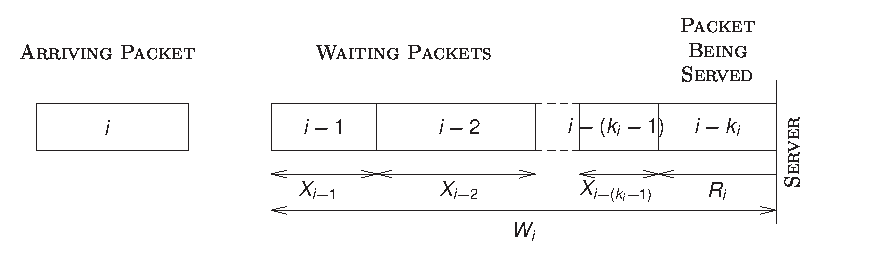
\includegraphics[%
  width=0.80\textwidth]{diagrams/residualServiceOverview.eps}\end{center}

In the diagram the $i$th arriving packet perceives a queueing time
of $W_{i}$ and a residual service time of $R_{i}$. The average residual
service time is the average $R_{i}$ for all packets. 

The assumptions used in deriving the formula are

\begin{itemize}
\item We assume that time averages are equivalent to steady state averages.
\item We assume that service times have a finite variance.
\item We assume that the arrival times are statistically independent of
the service times.
\item Assume the queue is FIFO.
\end{itemize}
\textbf{\emph{5 marks for each assumption, 10 marks for the description
of residual service time+diagram}}.

}{0}

\begin{qupart}
Use a graphical argument to derive a formula for the residual service
time. Combine this equation with the formula in part a) for the average
waiting time to show that\[
\bar{W}=\frac{\lambda\left\langle X^{2}\right\rangle }{2\left(1-\rho\right)},\]
where $\lambda$ is the arrival rate and $\left\langle X^{2}\right\rangle $
is the second moment of the service time distribution.

\mypercent{40}

\end{qupart}
\answer{


\subsection*{Answer}

We again turn to a graphical proof to obtain the value of the mean
residual service time. A plot can be drawn of the residual service
time over time.

\begin{center}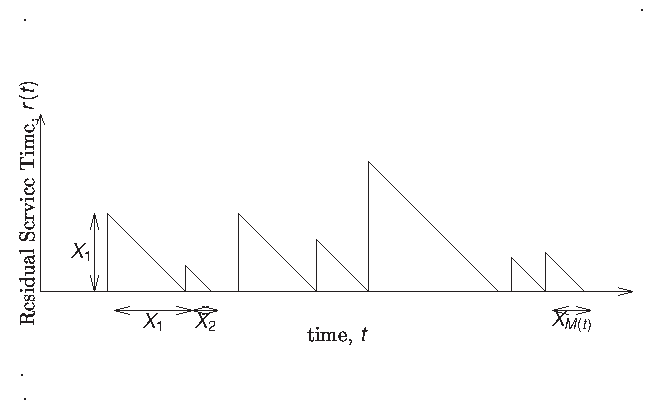
\includegraphics[%
  width=0.70\textwidth]{diagrams/residualTime.eps} \end{center}

$M\left(t\right)$ is the number of service completions in the interval
$[0,\, t]$.

The time average of the mean residual service time can then be calculated
in terms of the area under the curve, $A\left(t\right)$, which is
given by the area under each of the triangles,

\[
A(t)=\frac{1}{2}\sum_{i=1}^{M(t)}X_{i}^{2}.\]
 The average service time is the area divided by time, $t$, \begin{eqnarray*}
\frac{A(t)}{t} & = & \frac{M(t)}{t}\frac{A(t)}{M(t)}\\
 & = & \frac{1}{2}\frac{M(t)}{t}\frac{\sum_{i=1}^{M(t)}X_{i}^{2}}{M(t)}.\end{eqnarray*}
where we have used the number of arrivals after time $t$, as $M\left(t\right)$.
As $t\rightarrow\infty$, \emph{if the variance of the service time
distribution is finite}, we find that\[
\bar{R}=\frac{1}{2}\lambda\left\langle X^{2}\right\rangle .\]
 Again, assuming that time averages and ensemble averages are equal,
we substitute back into the equation provided in the previous part
to obtain the Pollaczek-Khinchin formula \[
\bar{W}=\frac{\lambda\left\langle X^{2}\right\rangle }{2(1-\rho)}.\]
\textbf{\emph{15 for the diagram, 10 for the area formula, 10 for
the introduction of $t$ and $M\left(t\right)$ and 5 for the right
answer.}} }{0}

\begin{qupart}
The equation you have derived is recognized as the Pollaczek-Khinchin
formula. Use it to derive the average waiting time in an $M/M/1$
queue.

\mypercent{15}

\end{qupart}
\answer{


\subsection*{Answer}

In an $M/M/1$ queue there is an exponential service time,\[
p\left(X\right)=\mu\exp\left(-\mu x\right).\]
The mean of this service time is $\left\langle X\right\rangle =\frac{1}{\mu}$
and the variance is $\textrm{var}\left(X\right)=\frac{1}{\mu^{2}}$.
Therefore the second moment is therefore\[
\left\langle X^{2}\right\rangle =\left\langle X\right\rangle ^{2}+\textrm{var}\left(X\right)=\frac{2}{\mu^{2}}.\]
Substituting into the Pollaczek-Khinchin formula we have\[
\bar{W}=\frac{\lambda}{\mu^{2}\left(1-\rho\right)}=\frac{\rho}{\mu\left(1-\rho\right)}\]
\textbf{\emph{5 marks for the distribution, 5 for the second moment
and 5 marks for the result}}}{0}

\begin{qupart}
Which service time distribution leads to the lowest delay for a given
mean? What characteristic of this distribution ensures it has the
lowest associated delay?

\mypercent{15}

\end{qupart}
\answer{


\subsection*{Answer}

The service time distribution that leads to the lowest delay for a
given mean $\bar{X}$ is the deterministic service time, \emph{i.e.}
an $M/D/1$ queue. This is because it is the distribution with the
lowest variance (the variance is zero) and therefore the second moment,
$\left\langle X^{2}\right\rangle =\bar{X}^{2}+\textrm{var}\left(X\right)$
is as low as it can be for this distribution (the variance cannot
be negative) which in turn means the average delay is as low as it
can be. There is no other distribution with a variance of zero. 

\textbf{\emph{5 marks for the right answer, and 10 marks for the fact
that it is the lowest variance}}.}{0}

\end{question}
~

\continued

\masters{\center{\Large\textbf{Section B}\normalsize}}{}

\begin{question}
This question focuses on the Erlang loss system
\begin{qupart}
Consider the Erlang B formula,\[
B(m,a)=\frac{\frac{a^{m}}{m!}}{\sum_{n=0}^{m}\frac{a^{n}}{n!}}.\]
What is the significance of the result of this formula? What do $a$
and $m$ stand for?

\mypercent{20}

\end{qupart}
\answer{


\subsection*{Answer}

The formula gives the blocking probability for the Erlang loss system.
$a=\frac{\lambda}{\mu}$ is the `offered load', a dimensionless constant
measured in Erlangs that gives the system load and $m$ is the number
of servers and the capacity of the system. \textbf{\emph{}}

\textbf{\emph{5 for a and m, 10 for the significance}} }{0}

\begin{qupart}
What problems might you have when trying to compute the result of
this formula on either a calculator or a computer? How would you seek
to solve these problems?

\mypercent{25}

\end{qupart}
\answer{ \textbf{\emph{}}


\subsection*{Answer}

For large values of $m$ there will be overflow problems for computing
$a^{m}$ and $m!$ This problem can be solved by computing the result
in log space and then exponentiating. To do this you use the log gamma
function for computing the factorial term (if they mention the use
of curves to solve the problems half marks for the solution part).

\textbf{\emph{15 for identifying the problem and 10 for identifiying
the solution.}{0}}}

\begin{qupart}
The steady state distribution for the Erlang loss system is given
by\[
P\left(k\right)=\frac{\frac{a^{k}}{k!}}{\sum_{n=0}^{m}\frac{a^{n}}{n!}}.\]
If the number of servers is very large ($m>>a)$ what will the average
number of customers in the system be?

\emph{Hint: consider what happens in the system as} $m\rightarrow\infty.$

\mypercent{25}

\end{qupart}
\answer{


\subsection*{Answer}

As the question states we should consider the limit as $m\rightarrow\infty$.
The steady state distribution for Erlang Loss is a truncated Poisson.
In the limit $m\rightarrow\infty$ (which is an $M/M/\infty$ queue),
the truncated Poisson becomes a Poisson distribution, \[
\sum_{n=0}^{\infty}\frac{a^{n}}{n!}=\exp\left(a\right),\]
so we have\[
P\left(k\right)=\frac{a^{k}}{k!}\exp\left(-a\right)\]
and the mean of this distribution is $\frac{1}{a}$.

\textbf{\emph{15 for determining that the system's steady state approximates
a Poisson for $m>>a$ (either by stating its originally a truncated
Poisson, or by producing the result for the infinte sum becoming an
exponential.) 10 for knowing (or proving!) that the mean of a Poisson
is $\frac{1}{a}$}}.}{0}

\begin{qupart}
The Erlang B formula is associated with the Erlang loss queueing system.
Under what conditions does the steady state distribution exist for
this queueing system? What is the form of this steady state distribution
when $a$ becomes much larger than $m$ and what is the resulting
effect on the carried load?
\end{qupart}

\mypercent{30}

~

\answer{


\subsection*{Answer }

The steady state \emph{always exists}. In some systems steady state
doesn't exist when the offered load, $a$, is higher than the number
of servers, $m$, however in the Erlang loss system the steady state
will converge towards $P\left(k\right)=1$ for $k=m$ and $P\left(k\right)=0$
otherwise. In this case most packets are rejected and the carried
load becomes very low. The steady state exists because the system
is lossy.

\textbf{\emph{5 marks for noting it always exists, 10 for giving the
form of the steady state and 5 for stating the carried load will be
small.}}

\textbf{\emph{}{0}}}~

\end{question}
\turnover

\begin{question}
\textbf{Annotate and hand in the Erlang C curves with your answer
to this question.}

United Telecom has just completed the purchase of several local telecommunications
companies, each with their own regional support teams. There are three
regional support teams. The number of staff in each team and the call
rate for each team's centre is given in the following table. 

\begin{center}\begin{tabular}{|c|c|c|c|}
\hline 
Region&
X&
Y&
Z\tabularnewline
\hline
\hline 
$m$&
12&
15&
8\tabularnewline
\hline
\hline 
customers/hour&
50&
70&
25\tabularnewline
\hline
\end{tabular}\end{center}

In the questions that follow you should assume that the call centres
can be accurately modelled as Erlang delay systems.
\begin{qupart}
Given that the average holding time, $\tau$, for support queries
is 6 minutes, use the Erlang C curves provided to give, for each region,
the probability of queueing, $C\left(m,a\right)$. 

\mypercent{30}

\end{qupart}
\answer{


\subsection*{Answer}

The offered load for this region is $a=\lambda\tau$, we have a holding
time of 6 minutes = 6/60 hours.

\begin{itemize}
\item Region X: $a_{X}=\frac{50\times6}{60}=\frac{30}{6}=5$ and $m=12$,
from Erlang C curves$C\left(12,5\right)=0.006$
\item Region Y: $a_{Y}=\frac{70\times6}{60}=\frac{42}{6}=7$ and $m=15$,
from Erlang C curves $C\left(15,7\right)=0.006$
\item Region Z: $a_{Z}=\frac{25\times6}{60}=\frac{15}{6}=2\frac{1}{2}$
and $m=8$, from Erlang C curves $C\left(8,2.5\right)=0.005$
\end{itemize}
Answers should also be marked on Erlang C curves.

\textbf{\emph{10}} \emph{}\textbf{\emph{for each probability of queueing.}}
}{0}

\begin{qupart}
The formula for the average queue length in the Erlang delay system
is\[
\bar{N}_{Q}=\frac{\rho}{1-\rho}C\left(m,a\right)\]
where $\rho$ is the queue utilization factor. Use Little's formula
to derive $\bar{W}$, the average queueing time, and use it compute
the expected queueing time for each call centre.

\mypercent{20}

\end{qupart}
\answer{

Little's formula for the queue is $\bar{N}_{Q}=\lambda\bar{W}$. So
this means that \[
\bar{W}=\frac{1}{\mu\left(1-\rho\right)}C\left(m,a\right)=\frac{1}{\mu\left(1-\frac{a}{m}\right)}C\left(m,a\right)\]
The queueing time for each centre is therefore

\begin{itemize}
\item Region X: $\bar{W}=\frac{1}{\frac{60}{6}\left(1-\frac{5}{12}\right)}C\left(12,5\right)=\frac{6}{35}\times0.006=8.57\times10^{-4}\textrm{hours}$
or about 3.7 seconds. 
\item Region Y: $\bar{W}=\frac{1}{\frac{60}{6}\left(1-\frac{7}{15}\right)}C\left(15,7\right)=\frac{3}{16}\times0.006=9.375\times10^{-4}$
hours or 4.05 seconds.
\item Region Z: $\bar{W}=\frac{1}{\frac{60}{6}\left(1-\frac{2.5}{8}\right)}C\left(8,2.5\right)=\frac{8}{55}\times0.005=6.060\times10^{-4}$
hours or 2.618 seconds. 
\end{itemize}
\textbf{\emph{5 for derivation of the formula and 5 for each answer.}}}{0}

\begin{qupart}
Show that the average queueing time for customers that queue is given
by\[
\bar{W}_{Q}=\frac{1}{\mu\left(1-\rho\right)}\]
and compute the average queue time for customers for each of the call
centres described above.

\mypercent{25}

\end{qupart}
\answer{


\subsection*{Answer}

The total queueing time is given by \[
\bar{W}=C\left(m,a\right)\bar{W}_{Q}+\left(1-C\left(m,a\right)\right)\bar{W}_{\sim Q}\]
where \begin{eqnarray*}
\bar{W}_{Q} & = & \textrm{queueing time for customers that queue}.\\
\bar{W}_{\sim Q} & = & \textrm{queueing time for customers that don't queue.}\end{eqnarray*}
Since $\bar{W}_{\sim Q}=0$ we can reorganise the formula as\[
\bar{W}_{Q}=\frac{\bar{W}}{C\left(m,a\right)}.\]
The queueing time for those that queue at each centre is therefore

\begin{itemize}
\item Region X: $\bar{W}=\frac{1}{\frac{60}{6}\left(1-\frac{5}{12}\right)}=\frac{6}{35}$
hour or 10.28 minutes.
\item Region Y: $\bar{W}=\frac{1}{\frac{60}{6}\left(1-\frac{7}{15}\right)}=\frac{15}{80}$
hour or 11.25 minutes.
\item Region Z: $\bar{W}=\frac{1}{\frac{60}{6}\left(1-\frac{2.5}{8}\right)}\frac{8}{55}$
hour or 8.73 minutes
\end{itemize}
\textbf{\emph{10 for the derivation of the formula and 5 for each
answer.}}}{0}

\begin{qupart}
The company wishes to cut costs by merging the call centres to one
location. Assuming that the total traffic level and the average holding
time remain the same, how many staff will be needed to keep the probability
of waiting at 0.006 or below?

\mypercent{5}

\end{qupart}
\answer{


\subsection*{Answer}

From the Erlang C curves, 26. 

\textbf{\emph{5 for the answer (should be indicated on the Erlang
C curves as well).}}}{0}

\begin{qupart}
Explain the difference in the number of staff required in the centralized
call centre in comparison to the three original call centres. In your
answer you should focus on the utilization factors in the two systems.

\mypercent{20}

\end{qupart}
\answer{


\subsection*{Answer}

The centralized system requires 9 fewer staff than the original three
separate systems for approximately the same performance. The reason
for this improved performance is the improved efficiency of the system.
In the original system the average efficiency can be found from the
utilization factors.

\begin{itemize}
\item Region X: $\rho_{X}=\frac{\lambda}{m}\tau=\frac{50\times6}{12\times60}=\frac{5}{12}$
\item Region Y: $\rho_{Y}=\frac{\lambda}{m}\tau=\frac{70\times6}{15\times60}=\frac{7}{15}$
\item Region Z: $\rho_{Z}=\frac{\lambda}{m}\tau=\frac{25\times6}{8\times60}=\frac{5}{16}$
\end{itemize}
so the average efficiency is $\frac{1}{3}\left(\frac{5}{12}+\frac{7}{15}+\frac{5}{16}\right)=0.399$\\
For the centralised system $m=26,$ $\lambda=50+70+25=145$ (by superposition
of Poissons), and $\tau=0.1$. So efficiency is\[
\rho=\frac{\lambda\tau}{m}=\frac{145\times0.1}{26}=0.557.\]
The second system is therfore more efficient which explains the reduction
in numbers of staff required.

\textbf{\emph{10 for the basic answer (i.e. the improved efficiency
of the system) and 10 for the actual figures.}}}{0}

\end{question}
~\continued

\begin{question}
You are presented with the following portion of Tcl code designed
for the network simulator NS2.
\begin{lyxcode}
set~node1~{[}\$ns~node{]}~\\
set~node2~{[}\$ns~node{]}~\\
set~node3~{[}\$ns~node{]}~\\
~\\
\$node1~set~multiPath\_~1~\\
~\\
set~link1~{[}\$ns~duplex-link~\$node1~\$node2~2Kb~0ms~DropTail{]}~\\
set~link2~{[}\$ns~duplex-link~\$node2~\$node3~2Kb~0ms~DropTail{]}~\\
set~link3~{[}\$ns~duplex-link~\$node1~\$node3~2Kb~0ms~DropTail{]}~\\
~\\
set~src~{[}new~Agent/UDP{]}~\\
\$ns~attach-agent~\$node1~\$src~\\
set~sink~{[}new~Agent/Null{]}~\\
\$ns~attach-agent~\$node3~\$sink~\\

\end{lyxcode}
\begin{qupart}
Assuming that only the specified nodes exist, draw the network topology
showing the associated routes.

\mypercent{25}

\end{qupart}
\answer{


\subsection*{Answer}

The \url{set link} statements give the structure of the network and
the \url{set src} and \url{set sink} statements along with the \url{set multiPath}
statment ensure that packets travel from \url{node1} to \url{node3}
along all possible routes. 

\begin{center}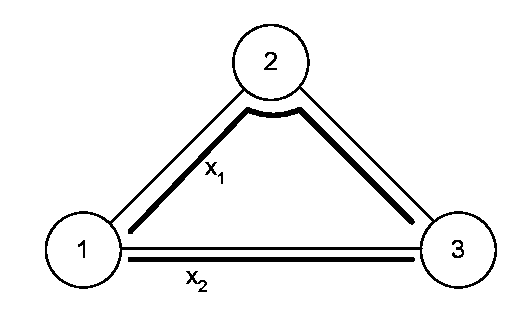
\includegraphics[%
  width=0.40\textwidth]{diagrams/ns2Network06.eps}\end{center}

In the diagram above we have omitted the arrows that show this, they
should either be shown or indicated in accompanying text.

\textbf{\emph{10 marks for the correct structure and 15 marks for
the correct routing information.}}

}{0}

\begin{qupart}
Packet arrivals occur as a Poisson distribution at \url{node1} with
a rate of 2 per second. Packet lengths are distributed as an exponential
distribution with a mean of 0.5 Kb. Assuming that packets are sent
randomly along all possible routes with equal probability, use Kleinrock's
independence assumption to estimate the steady state average number
of packets at each link and the average delay for each route.

\mypercent{25}

\end{qupart}
\answer{


\subsection*{Answer}

Packets arrive as a Poisson with a rate $\lambda=2$. They are sent
randomly along the two routes with equal probaility. This means, via
the decomposition property of Poisson processes, that the rate for
each route is $\lambda=2\times0.5=1$. The service time distribution
is dicated by the length of the packet and the bandwidth of the route.
The bandwidth (given in the code above) is 2Kb/s. Packet lengths are
0.5 Kb, so the service time distribution for all links will have $\mu=\frac{2}{0.4}=4$
packets/s. Kleinrock's independence assumption tells us to treat each
queue independently. The first route consists of two queues. 

The delay is given by the formula for the $M/M/1$ queue which is
\[
\bar{T}=\frac{1}{\mu-\lambda}=\frac{1}{4-1}=\frac{1}{3}s.\]
There are two queues in the first route so the total delay is $\frac{2}{3}s$. 

The calculation is the same for the second route, but there there
is only one queue (so in fact you don't need Kleinrock's assumption
--- see later question part) and the delay in the second route is
$\frac{1}{3}s$. \textbf{\emph{5 for decomposition of Poissons 10
for the correct formula and 5 for the correct answer for each route.}}}{0} 

\begin{qupart}
One of the routes in the network contains two queues. Explain how
the second queue's size, as perceived by an arriving packet, will
be related to the arriving packet's length. How will this waiting
time be affected for longer packets arriving at the second queue? 

\mypercent{20}

\end{qupart}
\answer{


\subsection*{Answer}

The longer packets will arrive at the second queue to find a shorter
queue than the shorter packets. Or in other words queue length at
the second queue are anti correlated with packet lengths. This is
because, while the longer packet was being served at the first queue
there is time for the second queue to empty out. This is analogous
to a slow moving truck driver who will generally see an open road
in front of him.

\textbf{\emph{10 marks for correctly saying that the queue will be
shorter for longer packets (or vice versa). 10 Marks for saying the
longer packet will wait less time at the second queue.}} 

}{0}

~

\begin{qupart}
For each route in the network consider the implications of Kleinrock's
independence assumption. For which route would you expect the assumption
to lead to more accurate results? Describe the reasoning behind your
answer.

\mypercent{20}

\end{qupart}
\answer{


\subsection*{Answer}

The second route which goes directly from node 1 to node 3 would be
much more accurate. This is because the assumptions behind Kleinrock
are valid for this route. The packet lengths are uncorrelated with
the arrival times. For the first route (via node 2) the packet lengths
become correlated through passing through the queue at node 2. 

\textbf{\emph{10 marks for the answer and 10 marks for the reasoning
(that independence holds for the second route.)}{0}}}

~

\begin{qupart}
Typically, in a large network, analytical modelling of the system
will not be possible. In practice we often turn to simulation for
modelling of such systems. Why might the sample-based approximations
to the system's characteristics we obtain from these simulations be
misleading?

\mypercent{10}

\end{qupart}
\answer{


\subsection*{Answer}

If the simulation is not run long enough it may not reach it's steady
state. It may even be hard to determine whether the system has a steady
state. If samples from the system are taken too close together in
time then they are not truly independent and sample based estimates
will be incorrect. \textbf{\emph{5 marks for steady state and 5 marks
for independence. Will also award 5 marks to answers that state you
need to obtain a lot of samples to get accurate results, but to get
10 you need to have both the first points as well.}{0}}}

\end{question}
\questionsend

\myfooter{}\newpage\myheader

\end{exam}
\topmargin -1.8cm {\bf\masters{COM6131}{COM3270}\hfill{\bf NETWORK PERFORMANCE ANALYSIS}\\\\\hspace{0.5cm}\raggedleft{{\bf Registration Number \rule{4cm}{.5pt}}}

\begin{center}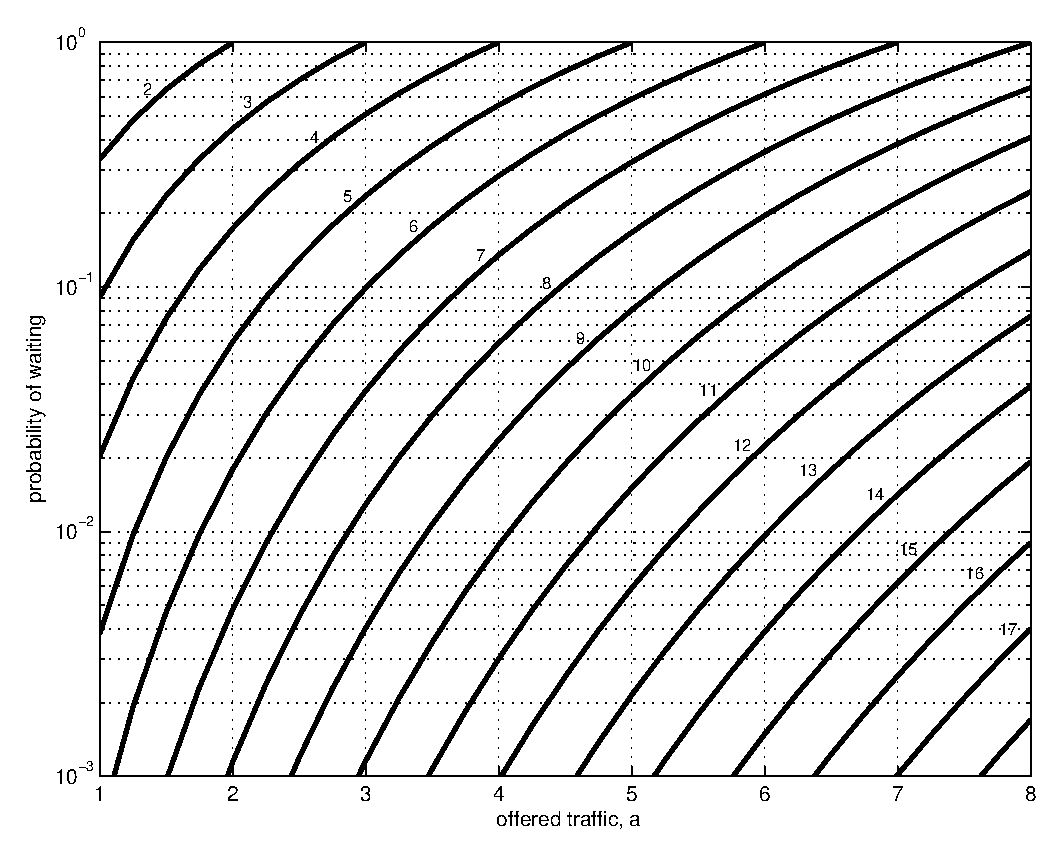
\includegraphics[%
  width=0.80\textwidth]{diagrams/erlangDelayCurves06.eps}\end{center}

\begin{center}\vspace{1cm}\end{center}

\begin{center}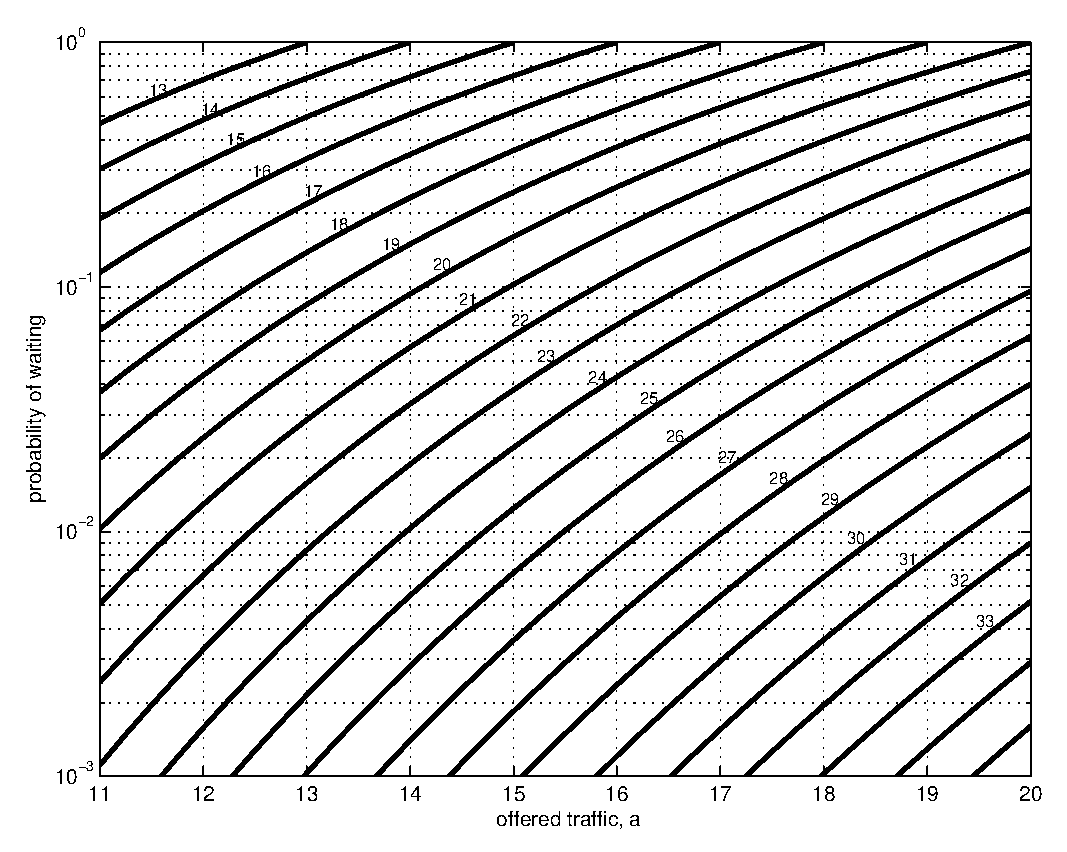
\includegraphics[%
  width=0.80\textwidth]{diagrams/erlangDelayCurves06_2.eps}\end{center}
\end{document}
